% Тип документа
\documentclass[a4paper,12pt]{extarticle}

% Шрифты, кодировки, символьные таблицы, переносы
\usepackage{cmap}
\usepackage[T2A]{fontenc}
\usepackage[utf8x]{inputenc}
\usepackage[russian]{babel}

% Это пакет -- хитрый пакет, он нужен но не нужен
\usepackage[mode=buildnew]{standalone}

\usepackage
	{
		% Дополнения Американского математического общества (AMS)
		amssymb,
		amsfonts,
		amsmath,
		amsthm,
		physics,
		% misccorr,
		% 
		% Графики и рисунки
		wrapfig,
		graphicx,
		subcaption,
		float,
		tikz,
		tikz-3dplot,
		caption,
		csvsimple,
		color,
		booktabs,
		pgfplots,
		pgfplotstable,
		geometry,
		% 
		% Таблицы, списки
		array,
		makecell,
		multirow,
		indentfirst,
		%
		% Интегралы и прочие обозначения
		ulem,
		esint,
		esdiff,
		% 
		% Колонтитулы
		fancyhdr,
	}  

\usepackage{xcolor}
\usepackage{hyperref}

 % Цвета для гиперссылок
\definecolor{linkcolor}{HTML}{000000} % цвет ссылок
\definecolor{urlcolor}{HTML}{799B03} % цвет гиперссылок
 
\hypersetup{pdfstartview=FitH,  linkcolor=linkcolor,urlcolor=urlcolor, colorlinks=true}
% Обводка текста в TikZ
\usepackage[outline]{contour}

% Увеличенный межстрочный интервал, французские пробелы
\linespread{1.3} 
\frenchspacing 

 
\usetikzlibrary
	{
		decorations.pathreplacing,
		decorations.pathmorphing,
		patterns,
		calc,
		scopes,
		arrows,
		fadings,
		through,
		shapes.misc,
		arrows.meta,
		3d,
		quotes,
		angles,
		babel
	}


\tikzset{
	force/.style=	{
		>=latex,
		draw=blue,
		fill=blue,
				 	}, 
	%				 	
	axis/.style=	{
		densely dashed,
		blue,
		line width=1pt,
		font=\small,
					},
	%
	th/.style=	{
		line width=1pt},
	%
	acceleration/.style={
		>=open triangle 60,
		draw=magenta,
		fill=magenta,
					},
	%
	inforce/.style=	{
		force,
		double equal sign distance=2pt,
					},
	%
	interface/.style={
		pattern = north east lines, 
		draw    = none, 
		pattern color=gray!60,
					},
	cross/.style=	{
		cross out, 
		draw=black, 
		minimum size=2*(#1-\pgflinewidth), 
		inner sep=0pt, outer sep=0pt,
					},
	%
	cargo/.style=	{
		rectangle, 
		fill=black!70, 
		inner sep=2.5mm,
					},
	%
	caption/.style= {
		midway,
		fill=white!20, 
		opacity=0.9
					},
	%
	}

\newenvironment{tikzpict}
    {
	    \begin{figure}[htbp]
		\centering
		\begin{tikzpicture}
    }
    { 
		\end{tikzpicture}
		% \caption{caption}
		% \label{fig:label}
		\end{figure}
    }


\newcommand{\vbLabel}[3]{\draw ($(#1,#2)+(0,5pt)$) -- ($(#1,#2)-(0,5pt)$) node[below]{#3}}
\newcommand{\vaLabel}[3]{\draw ($(#1,#2)+(0,5pt)$) node[above]{#3} -- ($(#1,#2)-(0,5pt)$) }

\newcommand{\hrLabel}[3]{\draw ($(#1,#2)+(5pt,0)$) -- ($(#1,#2)-(5pt,0)$) node[right, xshift=1em]{#3}}
\newcommand{\hlLabel}[3]{\draw ($(#1,#2)+(5pt,0)$) node[left, xshift=-1em]{#3} -- ($(#1,#2)-(5pt,0)$) }



\newcommand\zi{^{\,*}_i}
\newcommand\sumn{\sum_{i=1}^{N}}

\tikzset{
	coordsys/.style={scale=1.8,x={(1.1cm,-0cm)},y={(0.5cm,1cm)}, z={(0cm,0.8cm)}},
	coordsys/.style={scale=1.5,x={(0cm,0cm)},y={(1cm,0cm)}, z={(0cm,1cm)}}, 
	coordsys/.style={scale=1.5,x={(1cm,0cm)},y={(0cm,1cm)}, z={(0cm,0cm)}}, 
}

\usepgfplotslibrary{units}


% Draw line annotation
% Input:
%   #1 Line offset (optional)
%   #2 Line angle
%   #3 Line length
%   #5 Line label
% Example:
%   \lineann[1]{30}{2}{$L_1$}

\newcommand{\lineann}[4][0.5]{%
    \begin{scope}[rotate=#2, blue,inner sep=2pt, ]
        \draw[dashed, blue!40] (0,0) -- +(0,#1)
            node [coordinate, near end] (a) {};
        \draw[dashed, blue!40] (#3,0) -- +(0,#1)
            node [coordinate, near end] (b) {};
        \draw[|<->|] (a) -- node[fill=white, scale=0.8] {#4} (b);
    \end{scope}
}

\newcommand{\lineannn}[4][0.5]{%
    \begin{scope}[rotate=#2, blue,inner sep=2pt, ]
        \draw[dashed, blue!40] (0,0) -- +(0,#1)
            node [coordinate, near end] (a) {};
        \draw[dashed, blue!40] (#3,0) -- +(0,#1)
            node [coordinate, near end] (b) {};
        % \draw[color=white, color=blue] (a) -- node[fill=white, scale=0.8] {#4} (b);
        \draw[->|] (a)++(-0.3,0) -- (a);
        \draw[->|] (b)++(0.3,0) coordinate (xx) -- (b);
        \draw (xx) node[fill=white, scale=0.8, right] {#4};
    \end{scope}
}

% Круговая стрелка относительно центра (дуга из центра)
\tikzset{
  pics/carc/.style args={#1:#2:#3}{
    code={
      \draw[pic actions] (#1:#3) arc(#1:#2:#3);
    }
  },
  dash/.style={
  	dash pattern=on 5mm off 5mm
  }
}



\pgfplotsset{
    % most recent feature set of pgfplots
    compat=newest,
}

% const прямым шрифтом
\newcommand\ct[1]{\text{\rmfamily\upshape #1}}
\newcommand*{\const}{\ct{const}}


\usepackage[europeanresistors,americaninductors]{circuitikz}

% Style to select only points from #1 to #2 (inclusive)
\pgfplotsset{select/.style 2 args={
    x filter/.code={
        \ifnum\coordindex<#1\def\pgfmathresult{}\fi
        \ifnum\coordindex>#2\def\pgfmathresult{}\fi
    }
}}


\usepackage{array}
\usepackage{pstool}



\geometry		
	{
		left			=	2cm,
		right 			=	2cm,
		top 			=	3cm,
		bottom 			=	3cm,
		bindingoffset	=	0cm
	}

%%%%%%%%%%%%%%%%%%%%%%%%%%%%%%%%%%%%%%%%%%%%%%%%%%%%%%%%%%%%%%%%%%%%%%%%%%%%%%%

\fancyfoot{} 

\fancyfoot[C]{\thepage} 

%%%%%%%%%%%%%%%%%%%%%%%%%%%%%%%%%%%%%%%%%%%%%%%%%%%%%%%%%%%%%%%%%%%%%%%%%%%%%%%

\renewcommand{\contentsname}{Оглавление}

\usepackage{tocloft}
\renewcommand{\cftsecleader}{\cftdotfill{\cftdotsep}}
\usepackage{secdot}
\sectiondot{subsection}
% Тип документа

\begin{document}
% \begin{titlepage}

\begin{center}

{\small\textsc{Нижегородский государственный университет имени Н.\,И. Лобачевского}}
\vskip 1pt \hrule \vskip 3pt
{\small\textsc{Радиофизический факультет. Кафедра Электродинамики.}}

\vfill

{\Large Отчет по лабораторной работе №\labnumber\vskip 12pt\bfseries \labtheme}
	
\end{center}

\vfill
	
\begin{flushright}
	{Выполнили студенты \labgroup\ группы\\ \labauthors}%\vskip 12pt Принял:\\ Менсов С.\,Н.}
\end{flushright}
	
\vfill
	
\begin{center}
	Нижний Новгород, \the\year
\end{center}

\end{titlepage}


\begin{titlepage}
    \vspace*{\fill}
    \begin{center}
        \Huge \textbf{Определение коэффициента направленного действия рупорной антенны}
        \vskip 30pt \normalsize \textit{Описание лабораторной работы}
    \end{center}
    \vspace*{\fill}
\end{titlepage}

{\bfseries Цель работы:} 
Нахождение коэффициента направленного действия пирамидальной рупорной антенны с помощью так называемого зеркального
метода (метод Парселла).

\section{Теоритическая часть}

Антенна — устройство, предназначенное для излучения или приема волн (в нашем случае — электромагнитных). Одна из
важнейших функций антенны состоит в формировании излучения с определенными направленными свойствами. Основными
характеристиками направленности антенны являются диаграмма направленности (ДН) по амплитуде или по мощности, коэффициент
 направленного действия (КНД) и коэффициент усиления (КУ). Напомним, как вводятся эти характеристики.

\textit{Диаграмма направленности} по амплитуде есть угловое распределение амплитуды поля излучения, т.е. зависимость этой
амплитуды от полярного $\theta $ и азимутального $ \varphi $ углов при фиксированном расстоянии $r$ от антенны. \textit{Диаграмма направленности
по мощности} есть угловое распределение мощности излучения в единицу телесного угла $P(\theta, \varphi)=r^{2} S_{r}(r, \theta, \varphi)$,
где $S_{r}$ — радиальная компонента вектора Пойнтинга на достаточно большом расстоянии $r$ от антенны. Представляется 
удобным использование (наряду с абсолютной) нормированной диаграммы направленности $F(\theta,\varphi) = P(\theta,\varphi)/P(\theta_m,\varphi_m)$,
где $P(\theta_m,\varphi_m)$ — мощность, излучаемая в единичный телесный угол в направлении главного максимума $(\theta_m,\varphi_m)$ диаграммы
направленности. Диаграмму направленности изображают графически либо в виде <<объемной>>, рельефной картины, где по
каждому угловому направлению $(\theta,\varphi)$ откладывается величина, пропорциональная амплитуде поля излучения или излучаемой 
мощности (см. рис. \ref{fig:1:a}), либо с помощью плоской развертки отдельных, чаще всего двух ортогональных сечений, проходящих 
через направление главного максимума и векторы электрического \textbf{Е} и магнитного \textbf{Н} полей (см. рис.\ref{fig:1:b}). Поскольку основная
часть мощности, излучаемой направленной антенной, сосредоточена, как правило, в главном лепестке, то весьма показательной
представляется его угловая ширина, определяемая обычно по уровню половинной мощности $ \left(\Delta \theta_{0,5}\right) $, а иногда и по нулевому (или минимальному) значению
$ \left(\Delta \theta_{0}\right) $, как показано на рис.\ref{fig:1:b}. Диаграмма направленности антенны, характерный размер $l$
излучающей апертуры которой порядка или больше длины излучаемой волны $\lambda$, окончательно формируется в зоне Фраунгофера,
определяемой соотношением 

\begin{equation}
    r>>\frac{l^2}{\lambda}
    \label{eq:1}
\end{equation}

\textit{Коэффициент направленного действия} D характеризует
выигрыш по  мощности в направлении максимального излучения вследствие направленности антенны. Он равен отношению 
мощности, излучаемой в единицу телесного угла в направлении максимума диаграммы направленности $P(\theta_m,\varphi_m)$, к средней 
мощности $P_{cp} = P_{\text{изл}} /(4\pi)$, излучаемой антенной по всем направлениям, т.е. $ D=4 \pi
P\left(\theta_{m}, \varphi_{m}\right) / P_{\text{изл}} $, где $P_{\text{изл}} $ — полная излучаемая мощность:
$$  P_{\text{изл}} = \int_0^{2\pi}d\varphi \int_0^\pi P( \theta,\varphi ) \sin{\theta}d \theta. $$

Таким образом, имеем:
\begin{equation}
    D=\frac{4 \pi P\left(\theta_{m}, \varphi_{m}\right)}{\int_{0}^{\pi} d \varphi \int P(\theta, \varphi) \sin \theta d \theta}
    \label{eq:2}    
\end{equation}

\begin{center}
    \begin{figure}[h!]
        \begin{subfigure}[b]{.49\linewidth}
            \centering
            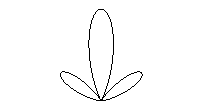
\includegraphics[width=\linewidth]{imgs/diag.pdf}
            \caption{}
            \label{fig:1:a}
        \end{subfigure}
        \begin{subfigure}[b]{.49\linewidth}
            \centering
            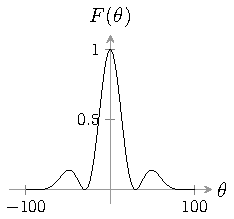
\includegraphics[width=\linewidth]{imgs/diag2.pdf}
            \caption{}
            \label{fig:1:b}
        \end{subfigure}
        \caption{Диаграмма направленности}
        \label{fig:1}
    \end{figure}
\end{center}

% \begin{center}
%     \begin{minipage}[t]{0.49\linewidth}
%         \includegraphics[width=\linewidth]{R1.png} 
%         \label{fig:1}
%         \vspace{-32pt}
%         \captionof{figure}{} 
%     \end{minipage}
%     \begin{minipage}[t]{0.49\linewidth}
%         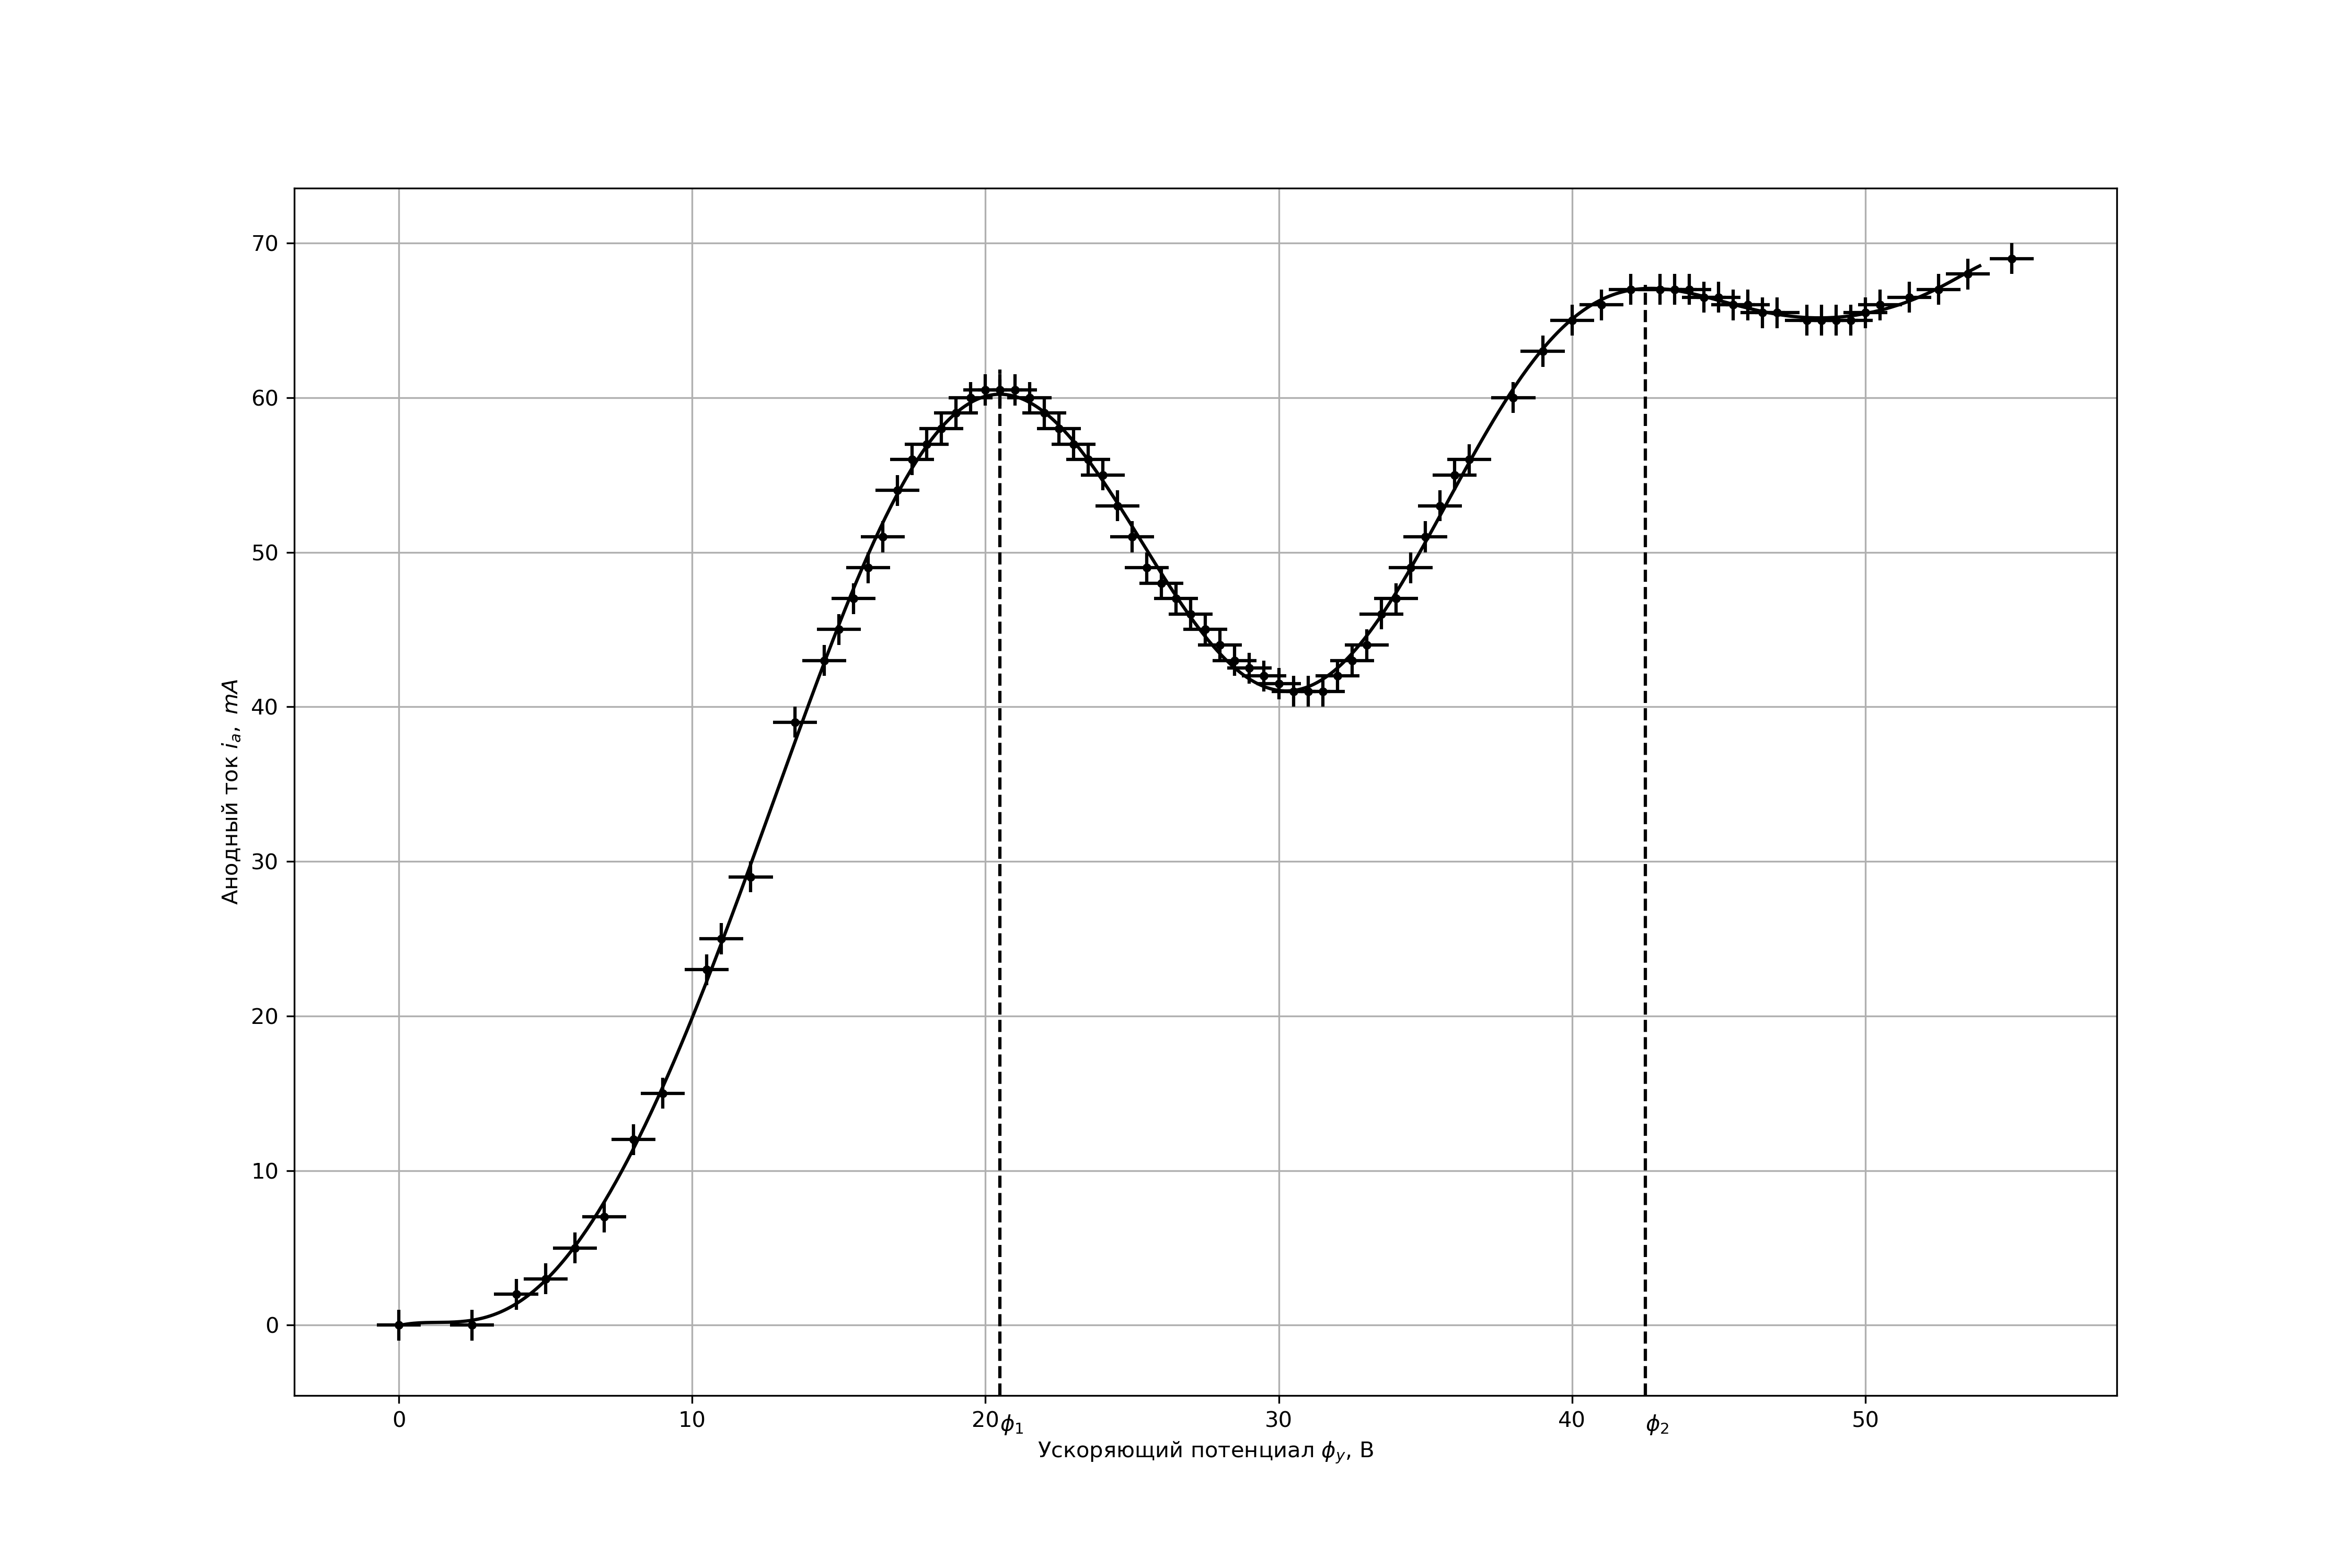
\includegraphics[width=\linewidth]{1.jpg} 
%         \label{fig:2}
%         \vspace{-32pt}
%         \captionof{figure}{} 
%     \end{minipage}
% \end{center}


\textit{Коэффициент усиления} G определяется как произведение КНД на коэффициент полезного действия (КПД) антенны $\eta$
(или, точнее, всего антенного тракта):

\begin{equation}
    G = D\eta
    \label{eq:3}    
\end{equation}

Этот последний коэффициент в свою очередь есть отношение полной мощности $P_{\text{изл}}$, излучаемой антенной, к полной
мощности $P_{\text{подв}}$, подводимой к антенне, т.е.
\begin{equation}
    \eta =\frac{P_{\text{изл}}}{P_{\text{подв}}} = \frac{\int_{0}^{2 \pi} d \varphi \int_{0}^{\pi} P(\theta, \varphi) \sin \theta d \theta}{P_{\text{подв}}}
    \label{eq:4}    
\end{equation}

В силу принципа взаимности ДН и КНД антенны при ее работе в режиме передачи и в режиме приема совпадают.

Для адекватного описания \textit{приемной антенны} вводятся некоторые дополнительные характеристики. 
Одна из основных таких характеристик — эффективная площадь приема антенны $A$.

\textit{Эффективная площадь} приема $A$ определяется как отношение полной принимаемой антенной мощности 
$P_{\text{пр}}$ к плотности потока падающего
излучения $S_n$ в месте расположения антенны:
\begin{equation}
    A = \frac{P_{np}}{S_n}
    \label{eq:5}
\end{equation}
Как показано в [1,2], величины $A$ и $D$ связаны соотношением
\begin{equation}
    A = \frac{\lambda^2}{4\pi}D.
    \label{eq:6}
\end{equation}

Цель настоящей работы заключается в экспериментальном определении КНД пирамидальной рупорной антенны с помощью так 
называемого зеркального метода (метода Парселла) и сравнении измеренного значения с рассчитанным теоретически. 
Зеркальный метод опирается на использование идеально (зеркально) отражающей плоской поверхности, расположенной в зоне 
Фраунгофера и ориентированной параллельно излучающей апертуре (см. рис. 2).

Согласно методу изображений отыскание отраженного поля, поступающего в антенну, сводится к нахождению поля, 
принимаемого от аналогичной зеркальной относительно отражающей плоскости излучающей антенны (рис. 2). В результате 
последовательного пересчета имеем: мощность, излучаемая гипотетической зеркальной антенной в единицу телесного угла 
в направлении на реальную антенну, равна $P_n = D P_{\text{изл}}/4\pi$, откуда плотность потока энергии в месте приема 
$S_n = P_n/4X^2 = D P_{\text{изл}}/(16\pi X^2)$, где $X$ — расстояние между антенной и отражающей плоскостью; наконец, 
мощность, принимаемая антенной, равна $P_{np} =A S_n =A D P_{\text{изл}}/(16\pi X^2)$. С учетом \ref{eq:6} окончательно 
получаем
\begin{equation}
    \frac{P_{np}}{P_{\text{изл}}} = \frac{D^2\lambda^2}{64\pi^2X^2}
    \label{eq:7}
\end{equation}

отсюда интересующая нас величина $D$ представляется в виде 
\begin{equation}
    D = \frac{8/pi X}{\lambda}\sqrt{\frac{P_{np}}{P_{\text{изл}}}}
    \label{eq:8}
\end{equation}

Таким образом, экспериментальное определение КНД требует нахождения отношения принимаемой зеркально отраженной мощности 
к мощности, излучаемой пирамидальной рупорной антенной. 

Измерительная установка включает генератор СВЧ диапазона (длина излучаемой волны $\lambda \approx$3 см) с отдельным 
блоком питания, волноводный тракт с измерительной линией и амперметром к ней, пирамидальный рупор, отражающий щи, 
щит с поглощающим покрытием. Блок-схема установки представлена на рис. 3. Отражающий щит должен располагаться в зоне 
Фраунгофера $X>>l_{1,2}^2/\lambda$ ($l_{1,2}$ — линейные размеры раскрыва рупора) и иметь линейные 
размеры $L_{1,2}$, позволяющие перекрывать основной лепесток диаграммы направленности:
 $ L_{1,2}>X \cdot \Delta \theta_{1,2} \approx X \cdot 2 \lambda / l_{1,2} (\Delta \theta_{1,2}$
— ширина основного лепестка в горизонтальной или вертикальной плоскости). Убедитесь, что эти условия выполнены! 
Установка позволяет контролируемо менять расстояние $X + \Delta X$ между антенной и отражательным щитом в пределах $\Delta X$ ~ 100 см. 
Следует особо подчеркнуть, что в измерительной линии используется квадратичный детектор, поэтому показания амперметра 
пропорциональны квадрату напряженности электрического поля в месте расположения зонда измерительной линии.

В согласованном (с хорошей точностью) режиме, когда отражение от конца волновода отсутствует, коэффициент отражения $\Gamma$ 
волны в волноводном тракте совпадает с членом $P_{np}/P_{\text{изл}}$ , содержащимся в \ref{eq:8}, и очевидным образом 
представляется через коэффициент бегущей волны (КБВ) в волноводе $\kappa = E_{min}/E_{max} (\Gamma= (1-\kappa)/(1+\kappa) )$, 
определяемый с помощью измерительной линии. Здесь $E_{min}, E_{max}$ — соответственно минимальное и максимальное значения 
поля в волноводном тракте. В результате получаем следующую формулу для КНД:
\begin{equation}
    D=\frac{8 \pi X}{\lambda} \frac{1-\kappa}{1+\kappa}
    \label{eq:9}
\end{equation}
Если детектор в измерительной линии квадратичный, то амперметр дает значения, пропорциональные $|E|^2$, так что вместо 
$\kappa$ измеряется величина $K = \kappa^2$; при этом вместо \ref{eq:9} нужно использовать выражение
\begin{equation}
    D=\frac{8 \pi X}{\lambda} \frac{1-\sqrt{K}}{1+\sqrt{K}}
    \label{eq:10}
\end{equation}
Итак, при наличии эффективного и надежного согласующего устройства отыскание КНД зеркальным методом сводится к 
процедуре согласования и последующего измерения КБВ в подводящем волноводном тракте. Согласование достигается за 
счет включения в волноводный тракт этого устройства (показано пунктиром на рис. 3) при использовании дополнительного 
щита с поглощающим покрытием, перехватывающего поле излучения (штрих-пунктирная линия на том же рисунке).

Вы будете работать в несогласованном режиме, когда согласующее устройство отсутствует и специальной процедуры 
согласования не проводится. С учетом отражения от конца подводящего тракта поле на оси волновода, отнормированное на 
амплитуду падающей волны, для некоторого фиксированного положения рупора запишется, очевидно, в виде
\begin{equation}
    E = 1e^{-ihx}+\Gamma_\kappa e^{i\varphi_\kappa} e^{ihx}+ \Gamma e^{e\varphi} e^{ihx}
    \label{eq:11}
\end{equation}
где $x$ - координата, отсчитываемая от конца волноводного тракта (см. рис. 4);$h$ — постоянная распространения волны в 
волноводе; $\Gamma_\kappa e^{i\varphi_\kappa}$ - коэффициент отражения от конца тракта; $\Gamma e^{e\varphi}$ — коэффициент 
отражения, обусловленный отражающим щитом. Выясните, на каком типе волны вы работаете и восстановите структуру 
электрического и магнитного полей в этой волне! Смещение антенны на величину $\Delta X$ приведет к появлению в последнем члене 
в \ref{eq:11} дополнительного множителя $ e^{ i k_0 2\Delta X } $ , связанного с дополнительным набегом фазы в свободном пространстве
($k_0=\omega/c$ — соответствующее волновое число). В результате для $ |E|^2 $ будем иметь
\begin{equation}
    \begin{aligned}
        |E|^{2} = &1+\Gamma_{\kappa}^{2}+\Gamma^{2}+2 \Gamma_{\kappa} \Gamma \cos {(\varphi-\varphi_{\kappa}+k_{0} 2 \Delta X)} +\\
        &+ 2 \Gamma_{\kappa} \cos{(2 h x+\varphi_{\kappa})}+2 \Gamma \cos{(2 h x+\varphi+k_{0} 2 \Delta X)}
    \end{aligned}
    \label{eq:12}
\end{equation}
Поскольку $ \Gamma_{\kappa} \text{и} \Gamma$ достаточно малы, то квадратичными величинами в первом приближении можно 
пренебречь, т.е. опустить второй, третий и четвертый члены в \ref{eq:12}; тогда эта формула упрощается к виду
\begin{equation}
    |E|^{2} \approx 1+2 \Gamma_{\kappa} \cos \left(2 h x+\varphi_{\kappa}\right)+2 \Gamma \cos \left(2 h x+\varphi+k_{0} 2 \Delta X\right)
    \label{eq:13}
\end{equation}
Все возможные способы определения КНД на данной установке опираются в той или иной степени на эту формулу. Два таких 
способа изложены в задании к работе. Попытайтесь предложить другие способы. Еще раз подчеркнем, что КНД однозначно 
определяется коэффициентом $\Gamma$:
\begin{equation}
    D = \frac{8 \pi X}{\lambda} \Gamma.
    \label{eq:14}
\end{equation}

\section{Задание}
\begin{enumerate}
    \item Помещая перед раскрывом рупора щит с поглощающим покрытием и убирая тем самым отраженное от металлического 
    щита поле $(\Gamma \approx 0)$, снимите распределение поля в волноводном тракте, т.е. зависимость $|E|^2(x)$ на оси волновода. 
    Определите значение коэффициента отражения от конца волновода $\Gamma_{\kappa}$ и оцените КПД системы, связанный с ее 
    недостаточным согласованием. По длине волны в волноводе $\lambda_{\text{в}}$ определите длину волны в свободном пространстве $\lambda$.
    \item Выберите такое положение $x$ зонда измерительной линии, при котором $\cos (2 h x +\varphi_{\kappa})$, и зафиксируйте его. 
    Уберите щит с поглощающим покрытием. Меняя затем положение антенны в пределах интервала, включающего несколько длин 
    волн, снимите зависимость $|E|^2(\Delta X)$. Определите значение коэффициента $\Gamma$, связанного с отражением от металлического 
    щита, и по нему КНД заданной пирамидальной рупорной антенны. Убедитесь, что величины $\Gamma_{\kappa}^2,\Gamma^2 $ и
    $\Gamma_{\kappa} \Gamma$ действительно достаточно малы. Выясните, как с помощью полученной зависимости можно 
    определить значение длины волны в свободном пространстве.
    \item Зафиксируйте положение антенны относительно металлического щита и определите отношение минимального $E_{min}$ 
    и максимального  $E_{max}$  значений поля в волноводном тракте: $\kappa = E_{min}/E_{max}$. Убедитесь, что эта 
    величина зависит от расстояния $X+\Delta X$ до щита. Меняя положение антенны, снимите зависимость
    $$ \tilde{\Gamma}(\Delta X)= \frac{1-\kappa (\Delta X)}{1+\kappa (\Delta X)} = \frac{1-\sqrt{K(\Delta X)}}{1+\sqrt{K(\Delta X)}} $$
    С помощью формулы \ref{eq:13} покажите, что максимальное значение $\Gamma$ приближенно равно $\tilde{\Gamma_{max}}
    \approx \Gamma + \Gamma_{\kappa}$. Учитывая это и используя найденное в п. 1 значение $\Gamma_{\kappa}$, определите 
    коэффициент $\Gamma$ и КНД антенны. Сопоставьте результаты с полученными ранее (п.2) и оцените погрешности обоих
    методов.
    \item Опираясь на электродинамическую формулировку принципа Гюйгенса [3] и используя кирхгофовское приближение для 
    задания поля на рас-крыве рупора, рассчитайте теоретически его КНД. При расчете воспользуйтесь дополнительным 
    упрощающим предположением о синфазности поля на раскрыве рупора. Подумайте, является ли в действительности данное 
    поле синфазным и как неоднородность фазы поля на раскрыве рупора сказывается на КНД.
    \item Сравните экспериментальные и теоретические результаты. Объясните причины возможных расхождений.
\end{enumerate}

\newpage
\begin{center}
    \section*{Литература}
\end{center}
\begin{enumerate}
    \item Айзенберг Г.З., Ямпольский В.Г., Терешин О.Н. Антенны УКВ. Ч.I. М.: Связь, 1977. Гл.8, §§8.2, 8.4; гл.12, 
    §§12.5,12.8; гл.16, §§16.1-16.4.
    \item Айзенберг Г.З. Антенны ультракоротких волн. М.: Связьиздат, 1957. Гл-VI, §§1,2; гл.VIII, §§2; гл.ХИ, §§4-7; гл.XVI, §§1-4.
    \item Вайнштейн Л.А. Электромагнитные волны. М.: Радио и связь, 1988. Гл. VII, §§38-41; гл. X, §§54-56; гл. XVII, §§92,93,95,98.    
\end{enumerate}

\end{document}